\subsection{Упражнение 1}

Пилообразный сигнал линейно нарастает от -1 до 1, а затем резко падает до -1 и повторяется.

\noindent Напишите класс, называемый SawtoothSignal, расширяющий signal и предоставляющий evaluate для оценки пилообразного сигнала.

\noindent Вычислите спектр пилообразного сигнала. Как соотносится его гармоническая структура с тругольными с прямоугольными сигналами?

Напишем класс пилообразного сигнала:

\begin{lstlisting}[language=Python]
class SawtoothSignal(Sinusoid):

  def evaluate(self,ts):
    cycles = self.freq * ts + self.offset / (pi / 2)
    frac, _ = np.modf(cycles)
    u = unbias(frac)
    high, low = abs(max(u)), abs(min(u))
    ys = self.amp * u / max(high,low)
    return ys
\end{lstlisting}

Проверим график:

\begin{lstlisting}[language=Python]
saw_signal = SawtoothSignal(200)
saw_signal.plot()
\end{lstlisting}

\begin{figure}[H]
	\begin{center}
		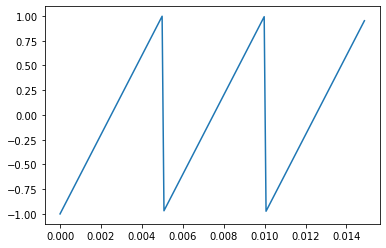
\includegraphics[scale=1]{fig/lab02/lab02_5_0.png}
		\caption{График пилообразного сигнала}
	\end{center}
\end{figure}

Сделаем экземпляр класса Wave для построения спектра сигнала.

\begin{lstlisting}[language=Python]
saw_spectrum = saw_signal.make_wave(duration = 0.5).make_spectrum()
saw_spectrum.plot()
\end{lstlisting}

\begin{figure}[H]
	\begin{center}
		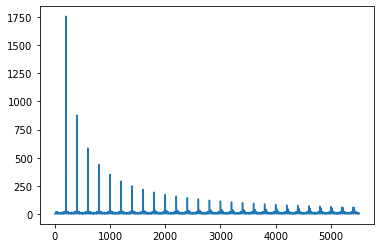
\includegraphics[scale=1]{fig/lab02/lab02_7_0.png}
		\caption{Спектр пилообразного сигнала}
	\end{center}
\end{figure}

Добавим прямоугольный сигнал:

\begin{lstlisting}[language=Python]
from thinkdsp import SquareSignal

squar_signal = SquareSignal(amp = 0.25)
squar_signal.plot()
\end{lstlisting}

\begin{figure}[H]
	\begin{center}
		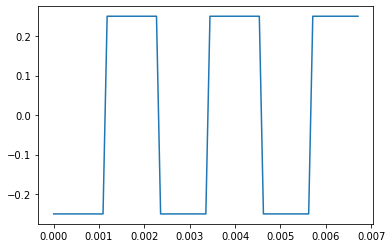
\includegraphics[scale=1]{fig/lab02/lab02_9_0.png}
		\caption{График прямоугольного сигнала}
	\end{center}
\end{figure}

\begin{lstlisting}[language=Python]
squar_spectrum = squar_signal.make_wave().make_spectrum()
squar_spectrum.plot()
\end{lstlisting}

\begin{figure}[H]
	\begin{center}
		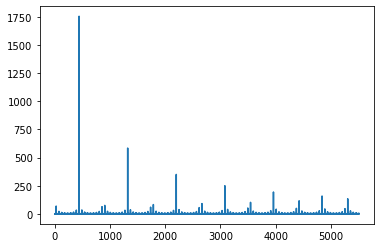
\includegraphics[scale=1]{fig/lab02/lab02_10_0.png}
		\caption{Спектр прямоугольного сигнала}
	\end{center}
\end{figure}

Также добавим треугольный сигнал:

\begin{lstlisting}[language=Python]
from thinkdsp import TriangleSignal

tri_signal = TriangleSignal(amp = 0.5)
tri_signal.plot()
\end{lstlisting}

\begin{figure}[H]
	\begin{center}
		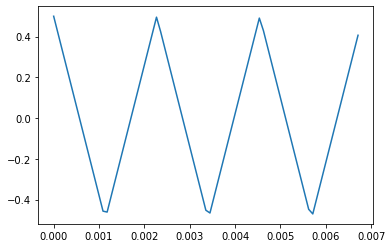
\includegraphics[scale=1]{fig/lab02/lab02_12_0.png}
		\caption{График треугольного сигнала}
	\end{center}
\end{figure}

\begin{lstlisting}[language=Python]
tri_spectrum = tri_signal.make_wave().make_spectrum()
tri_spectrum.plot()
\end{lstlisting}

\begin{figure}[H]
	\begin{center}
		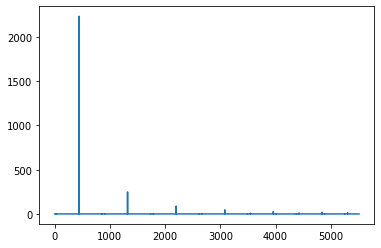
\includegraphics[scale=1]{fig/lab02/lab02_13_0.png}
		\caption{Спектр треугольного сигнала}
	\end{center}
\end{figure}

По сравнению с квадратным сигналом, пилообразный включает в себя четные и нечётные гармоники. Но оба сигнала снижают амплитуду обратно пропорциально частоте.
По сравнению с треугольным сигналом, треугольный сигнал падает $1/f^2$, а пилообразный $1/f$.

\subsection{Упражнение 2}

Создайте прямугольный сигнал 1100 Гц и вычислите wave с выборками 10 000 кадров в секунду. Постройте спектр и убедитесь, что большинство гармоник "завёрнуты" из-за биений, слышно ли последствия этого при проигрывании?

\begin{lstlisting}[language=Python]
square_signal = SquareSignal(freq=1500)
square_wave = square_signal.make_wave(duration = 1, framerate = 10000)
square_wave.make_spectrum().plot()
\end{lstlisting}

\begin{figure}[H]
	\begin{center}
		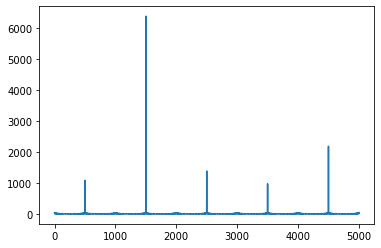
\includegraphics[scale=1]{fig/lab02/lab02_16_0.png}
		\caption{Спектр сигнала с биениями}
	\end{center}
\end{figure}

По спекторграмме видим, что из-за выбранного фреймрейта 10000 у нас начинаются биения. Сигналы больших частот закольцовываются вокруг 5000Гц и 0Гц.

Когда мы слушаем получившийся звук, мы слышим основную частоту на 500Гц.

\begin{lstlisting}[language=Python]
s1 = square_wave.make_spectrum()
s1.high_pass(1000)
s1.plot()
\end{lstlisting}

\begin{figure}[H]
	\begin{center}
		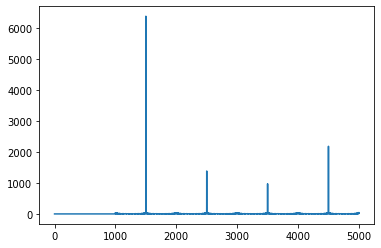
\includegraphics[scale=1]{fig/lab02/lab02_20_0.png}
		\caption{Спектр сигнала с фильтром}
	\end{center}
\end{figure}

Звук отличается, значит действительно, мы слышим звук частотой 500Гц.

\subsection{Упражнение 3}

Возьмите объект спектра spectrum, и выведите первые несколько значений spectrum.fs, вы увидите, что частоты начинаются с нуля. Итак, «spectrum.hs[0]» — это величина компонента с частотой 0. Но что это значит?

\noindent Попробуйте этот эксперимент:

1. Сделать треугольный сигнал с частотой 440 и создать Волну длительностью 0,01 секунды. Постройте форму волны.

2. Создайте объект Spectrum и напечатайте spectrum.hs[0]. Каковы амплитуда и фаза этой составляющей?

3. Установите spectrum.hs[0] = 100. Создайте волну из модифицированного спектра и выведите ее. Как эта операция влияет на форму сигнала?


\begin{lstlisting}[language=Python]
trian_signal = TriangleSignal(freq=440)
trian_wave = trian_signal.make_wave(duration = 0.01)
trian_wave.plot()
\end{lstlisting}

\begin{figure}[H]
	\begin{center}
		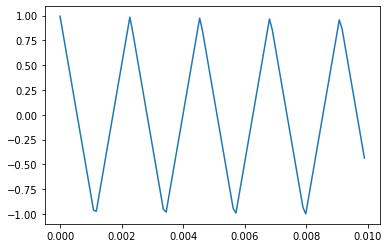
\includegraphics[scale=1]{fig/lab02/lab02_24_0.png}
		\caption{График сигнала}
	\end{center}
\end{figure}

Проверим что лежит в 0 элементе чисел спекторграммы

\begin{lstlisting}[language=Python]
trian_spectrum = trian_wave.make_spectrum()
trian_spectrum.hs[0]
\end{lstlisting}

\begin{lstlisting}
(1.0436096431476471e-14+0j)
\end{lstlisting}
Видим комплексное число, с 0 мнимой частью. Сам элемент очень близок к нулю.

\begin{lstlisting}[language=Python]
trian_spectrum.hs[0] = 100
trian_wave = trian_spectrum.make_wave()
trian_wave.plot()
\end{lstlisting}

\begin{figure}[H]
	\begin{center}
		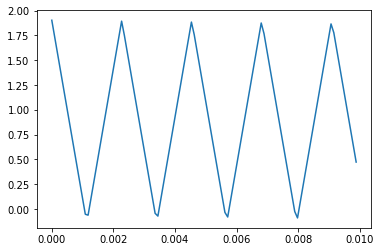
\includegraphics[scale=1]{fig/lab02/lab02_28_0.png}
		\caption{График сигнала с изменённым нулевым числом спекторграммы}
	\end{center}
\end{figure}

Можно заметить, что сигнал сместился по вертикали вверх. Следовательно от первого элемента зависит смещение сигнала. Т.к. сначала элемент был близок к нулю, то нулевой элемент это сигнал без смещения.

\subsection{Упражнение 4}

Напишите функцию, которая принимает Spectrum в качестве параметра и модифицирует его, деля каждый элемент hs на соответствующую частоту из fs. Протестируйте свою функцию, используя один из файлов WAV в репозитории или любой объект Wave.

1. Рассчитайте спектр и начертите его.

2. Измените спектр, используя свою функцию, и снова начертите его.

3. Сделать волну из модифицированного Spectrum и прослушать ее. Как эта операция влияет на сигнал?


Исходя из последнего пункта первый элемент очень близок к нулю. Поэтому на него делить не надо, а то получим очень большие значения (на самом деле я понял это после запуска программы из-за ошибок при делении на ноль).

\begin{lstlisting}[language=Python]
def spectrum_divider(spectrum):
    spectrum.hs[1:] /= spectrum.fs[1:]
    spectrum.hs[0] = 0
\end{lstlisting}

\begin{lstlisting}[language=Python]
if not os.path.exists('164718__bradovic__piano.wav'):
    !wget https://github.com/wooftown/spbstu-telecom/raw/main/Content/164718__bradovic__piano.wav
    
wave = read_wave('164718__bradovic__piano.wav').segment(18.3,0.5)
wave.make_audio()
wave.make_spectrum().plot(high = 5000)
\end{lstlisting}

\begin{figure}[H]
	\begin{center}
		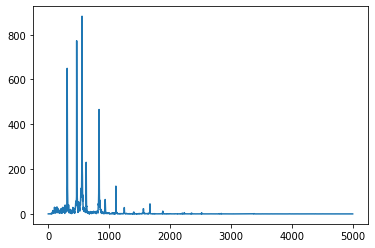
\includegraphics[scale=1]{fig/lab02/lab02_35_0.png}
		\caption{Спектр сигнала}
	\end{center}
\end{figure}

\begin{lstlisting}[language=Python]
sp = wave.make_spectrum()
spectrum_divider(sp)
sp.plot(high = 5000)
\end{lstlisting}

\begin{figure}[H]
	\begin{center}
		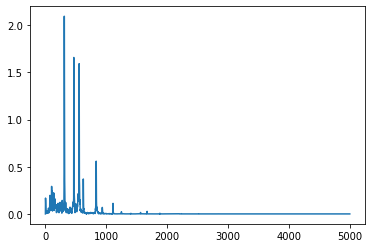
\includegraphics[scale=1]{fig/lab02/lab02_36_0.png}
		\caption{Спектр изменённого сигнала}
	\end{center}
\end{figure}

Видим. что ампилутуда очень поменялась, а частоты стоящие ближе к 0 Гц стали больше, чем следующие, что понятно. На выходе получилось, что полученный звук звучит более чисто, из-за фильтрации высоких частот.

\subsection{Упражнение 5}

Треугольные и прямоугольные волны имеют только нечетные гармоники; пилообразная волна имеет как четные, так и нечетные гармоники. Гармоники прямоугольной и пилообразной волн затухают пропорционально $1/f$; гармоники треугольной волны затухают как $1/f^2$. Можете ли вы найти форму волны, в которой четные и нечетные гармоники затухают как $1/f^2$?

\noindent Подсказка: есть два способа подойти к этому: вы можете построить нужный сигнал путем сложения синусоид, или вы может начаться с сигнала, похожего на то, что вы хотите, и изменить его.


\noindent Не зря мы писали предыдущую функцию, поэтому возьмём пилообразный сигнал который имеет и четные и нечётные гармоники, а потом применим нашу функцию.

\begin{lstlisting}[language=Python]
saw_signal = SawtoothSignal(500)
saw_spectrum = saw_signal.make_wave().make_spectrum()
saw_spectrum.plot()
\end{lstlisting}

\begin{figure}[H]
	\begin{center}
		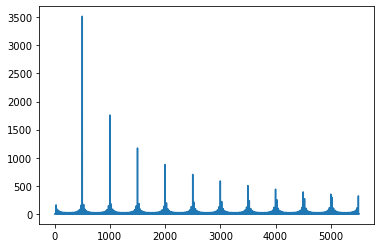
\includegraphics[scale=1]{fig/lab02/lab02_42_0.png}
		\caption{Спектр пилообразного сигнала}
	\end{center}
\end{figure}

\begin{lstlisting}[language=Python]
saw_spectrum1 =  saw_signal.make_wave().make_spectrum()
spectrum_divider(saw_spectrum1)
saw_spectrum1.plot()
\end{lstlisting}

\begin{figure}[H]
	\begin{center}
		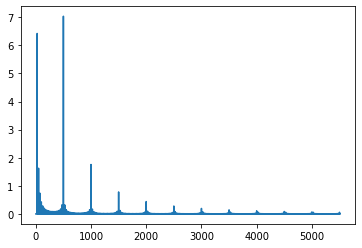
\includegraphics[scale=1]{fig/lab02/lab02_43_0.png}
		\caption{Спектр пилообразного сигнала}
	\end{center}
\end{figure}

Тут получилось, что амплитуда у 0 слишком большая, исправим изменив параметры.

\begin{lstlisting}[language=Python]
saw_signal = SawtoothSignal(freq=freq)
saw_wave = saw_signal.make_wave(duration=1, framerate=10000)
saw_spectrum = saw_wave.make_spectrum()
saw_spectrum.plot()
saw_spectrum1 = saw_wave.make_spectrum()
spectrum_divider(saw_spectrum1)
saw_spectrum1.plot()
\end{lstlisting}

\begin{figure}[H]
	\begin{center}
		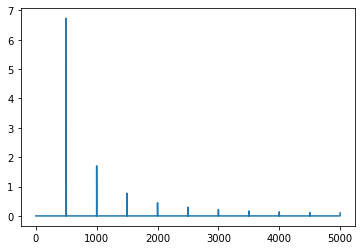
\includegraphics[scale=1]{fig/lab02/lab02_47_0.png}
		\caption{Спектр необходимого сигнала}
	\end{center}
\end{figure}

Теперь нам интересно какой получился график:

\begin{lstlisting}[language=Python]
saw_spectrum1.make_wave().segment(duration = 0.005).plot()
\end{lstlisting}

\begin{figure}[H]
	\begin{center}
		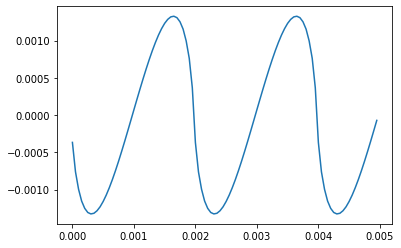
\includegraphics[scale=1]{fig/lab02/lab02_49_0.png}
		\caption{График необходимого сигнала}
	\end{center}
\end{figure}

Сигнал немного напоминает синусойду, но она как-будто немного наклонена.

\subsection{Вывод}

В данной работе были исследованы некоторые виды сигналов. Были рассмотрены спектры и гармонические структуры сигналов. Также в одном из пунктов были замечены биения и мы проверили их действие на звук.